% Options for packages loaded elsewhere
\PassOptionsToPackage{unicode}{hyperref}
\PassOptionsToPackage{hyphens}{url}
\PassOptionsToPackage{dvipsnames,svgnames,x11names}{xcolor}
%
\documentclass[
  letterpaper,
  DIV=11,
  numbers=noendperiod]{scrartcl}

\usepackage{amsmath,amssymb}
\usepackage{iftex}
\ifPDFTeX
  \usepackage[T1]{fontenc}
  \usepackage[utf8]{inputenc}
  \usepackage{textcomp} % provide euro and other symbols
\else % if luatex or xetex
  \usepackage{unicode-math}
  \defaultfontfeatures{Scale=MatchLowercase}
  \defaultfontfeatures[\rmfamily]{Ligatures=TeX,Scale=1}
\fi
\usepackage{lmodern}
\ifPDFTeX\else  
    % xetex/luatex font selection
  \setmainfont[]{Inter}
  \setsansfont[]{Inter}
  \setmathfont[]{Fira Math}
\fi
% Use upquote if available, for straight quotes in verbatim environments
\IfFileExists{upquote.sty}{\usepackage{upquote}}{}
\IfFileExists{microtype.sty}{% use microtype if available
  \usepackage[]{microtype}
  \UseMicrotypeSet[protrusion]{basicmath} % disable protrusion for tt fonts
}{}
\makeatletter
\@ifundefined{KOMAClassName}{% if non-KOMA class
  \IfFileExists{parskip.sty}{%
    \usepackage{parskip}
  }{% else
    \setlength{\parindent}{0pt}
    \setlength{\parskip}{6pt plus 2pt minus 1pt}}
}{% if KOMA class
  \KOMAoptions{parskip=half}}
\makeatother
\usepackage{xcolor}
\usepackage{soul}
\setlength{\emergencystretch}{3em} % prevent overfull lines
\setcounter{secnumdepth}{5}
% Make \paragraph and \subparagraph free-standing
\ifx\paragraph\undefined\else
  \let\oldparagraph\paragraph
  \renewcommand{\paragraph}[1]{\oldparagraph{#1}\mbox{}}
\fi
\ifx\subparagraph\undefined\else
  \let\oldsubparagraph\subparagraph
  \renewcommand{\subparagraph}[1]{\oldsubparagraph{#1}\mbox{}}
\fi


\providecommand{\tightlist}{%
  \setlength{\itemsep}{0pt}\setlength{\parskip}{0pt}}\usepackage{longtable,booktabs,array}
\usepackage{calc} % for calculating minipage widths
% Correct order of tables after \paragraph or \subparagraph
\usepackage{etoolbox}
\makeatletter
\patchcmd\longtable{\par}{\if@noskipsec\mbox{}\fi\par}{}{}
\makeatother
% Allow footnotes in longtable head/foot
\IfFileExists{footnotehyper.sty}{\usepackage{footnotehyper}}{\usepackage{footnote}}
\makesavenoteenv{longtable}
\usepackage{graphicx}
\makeatletter
\def\maxwidth{\ifdim\Gin@nat@width>\linewidth\linewidth\else\Gin@nat@width\fi}
\def\maxheight{\ifdim\Gin@nat@height>\textheight\textheight\else\Gin@nat@height\fi}
\makeatother
% Scale images if necessary, so that they will not overflow the page
% margins by default, and it is still possible to overwrite the defaults
% using explicit options in \includegraphics[width, height, ...]{}
\setkeys{Gin}{width=\maxwidth,height=\maxheight,keepaspectratio}
% Set default figure placement to htbp
\makeatletter
\def\fps@figure{htbp}
\makeatother

\usepackage{amsmath, xparse}
\usepackage{fancyvrb, fvextra}
\usepackage{unicode-math}
\usepackage{svg}
\usepackage{multicol}
\usepackage{listings}
\usepackage{systeme}
\usepackage{xifthen}
\DefineVerbatimEnvironment{Highlighting}{Verbatim}{breaklines,commandchars=\\\{\}}
\lstset{basicstyle=\ttfamily\footnotesize,breaklines=true}
\newcommand\rowop[1]{\scriptstyle\smash{\xrightarrow[\vphantom{#1}]{\mkern-4mu#1\mkern-4mu}}}
\DeclareDocumentCommand\converttorows%
{>{\SplitList{,}}m}%
{\ProcessList{#1}{\converttorow}}
\NewDocumentCommand{\converttorow}{m}
{\ifthenelse{\isempty{#1}}{}{\rowop{#1}}\\}

\DeclareDocumentCommand \rowops{m}
{\;
\begin{matrix}
\converttorows {#1}
\end{matrix}
\; }
\KOMAoption{captions}{tableheading}
\makeatletter
\makeatother
\makeatletter
\makeatother
\makeatletter
\@ifpackageloaded{caption}{}{\usepackage{caption}}
\AtBeginDocument{%
\ifdefined\contentsname
  \renewcommand*\contentsname{Table of contents}
\else
  \newcommand\contentsname{Table of contents}
\fi
\ifdefined\listfigurename
  \renewcommand*\listfigurename{List of Figures}
\else
  \newcommand\listfigurename{List of Figures}
\fi
\ifdefined\listtablename
  \renewcommand*\listtablename{List of Tables}
\else
  \newcommand\listtablename{List of Tables}
\fi
\ifdefined\figurename
  \renewcommand*\figurename{Figure}
\else
  \newcommand\figurename{Figure}
\fi
\ifdefined\tablename
  \renewcommand*\tablename{Table}
\else
  \newcommand\tablename{Table}
\fi
}
\@ifpackageloaded{float}{}{\usepackage{float}}
\floatstyle{ruled}
\@ifundefined{c@chapter}{\newfloat{codelisting}{h}{lop}}{\newfloat{codelisting}{h}{lop}[chapter]}
\floatname{codelisting}{Listing}
\newcommand*\listoflistings{\listof{codelisting}{List of Listings}}
\makeatother
\makeatletter
\@ifpackageloaded{caption}{}{\usepackage{caption}}
\@ifpackageloaded{subcaption}{}{\usepackage{subcaption}}
\makeatother
\makeatletter
\@ifpackageloaded{tcolorbox}{}{\usepackage[skins,breakable]{tcolorbox}}
\makeatother
\makeatletter
\@ifundefined{shadecolor}{\definecolor{shadecolor}{rgb}{.97, .97, .97}}
\makeatother
\makeatletter
\makeatother
\makeatletter
\makeatother
\ifLuaTeX
  \usepackage{selnolig}  % disable illegal ligatures
\fi
\IfFileExists{bookmark.sty}{\usepackage{bookmark}}{\usepackage{hyperref}}
\IfFileExists{xurl.sty}{\usepackage{xurl}}{} % add URL line breaks if available
\urlstyle{same} % disable monospaced font for URLs
\hypersetup{
  colorlinks=true,
  linkcolor={blue},
  filecolor={Maroon},
  citecolor={Blue},
  urlcolor={Blue},
  pdfcreator={LaTeX via pandoc}}

\author{}
\date{}

\begin{document}
\begin{titlepage}

    \newcommand{\HRule}{\rule{\linewidth}{0.5mm}}
    
    \center
    
    \vspace{10cm}

    \textsc{\LARGE Gwinnett School of Math, Science, and Technology }\\[0.3cm]
    
    \vspace{0.5cm}

    \HRule \\[0.4cm]
    { \huge \bfseries Multivariable Calculus Yearlong Notes}\\[0.03cm]
    \HRule \\[1.5cm]
    
    \begin{minipage}{0.4\textwidth}
    \begin{flushleft} \Large
    Anish Goyal \\5th Period
    \end{flushleft}
    \end{minipage}
    ~
    \begin{minipage}{0.4\textwidth}
    \begin{flushright} \Large
    Donny Thurston\\Educator
    \end{flushright}
    \end{minipage}\\[1cm]
    
    {\huge 2023-2024}\\[1cm]
    
    
\includegraphics{img/logo.png}\\
    \vfill
    \end{titlepage}
\newpage

\ifdefined\Shaded\renewenvironment{Shaded}{\begin{tcolorbox}[interior hidden, frame hidden, borderline west={3pt}{0pt}{shadecolor}, boxrule=0pt, breakable, sharp corners, enhanced]}{\end{tcolorbox}}\fi

\renewcommand*\contentsname{Table of Contents}
{
\hypersetup{linkcolor=}
\setcounter{tocdepth}{4}
\tableofcontents
}
\newpage{}

\hypertarget{systems-of-linear-equations-and-matrices}{%
\section{Systems of Linear Equations and
Matrices}\label{systems-of-linear-equations-and-matrices}}

\hypertarget{matrix-operations}{%
\subsection{Matrix Operations}\label{matrix-operations}}

\begin{itemize}
\tightlist
\item
  Matrix operations are given as: rows x columns
\item
  Two matrices are equal \(\iff\) they have the same dimensions and
  values
\end{itemize}

\hypertarget{addition-subtraction}{%
\subsubsection{Addition \& Subtraction}\label{addition-subtraction}}

Two matrices can be added/subtracted \(\iff\) they have the same
dimensions. 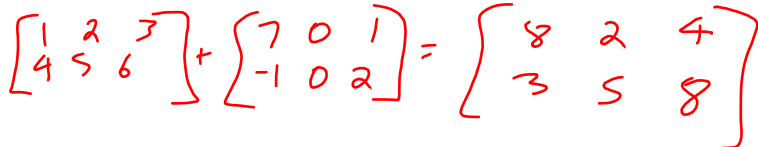
\includegraphics{img/addition-subtraction.png}

\hypertarget{scalar-multiplication}{%
\subsubsection{Scalar Multiplication}\label{scalar-multiplication}}

\begin{itemize}
\tightlist
\item
  Scalar multiplication is defined as multiplying each element of a
  matrix by a number 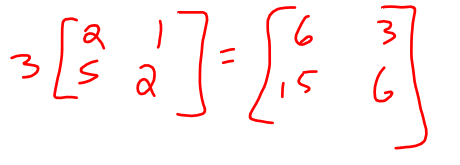
\includegraphics{img/scalar.png}
\end{itemize}

\hypertarget{matrix-multiplication}{%
\subsubsection{Matrix Multiplication}\label{matrix-multiplication}}

\begin{itemize}
\tightlist
\item
  We can \textbf{only} multiply an (m x n) by (n x p) matrix.
\item
  The resulting matrix will be (m x p)
\end{itemize}

\hypertarget{properties-of-matrix-arithmetic}{%
\subsubsection{Properties of Matrix
Arithmetic}\label{properties-of-matrix-arithmetic}}

\begin{enumerate}
\def\labelenumi{(\alph{enumi})}
\tightlist
\item
  \(A + B = B + A\) \textbf{(Commutative law for addition)}
\item
  \(A + (B + C) = (A + B) + C\) \textbf{(Associative law for addition)}
\item
  \(A(BC) = (AB)C\) \textbf{(Associative law for multiplication)}
\item
  \(A(B+C) = AB + AC\) \textbf{(Left distributive law)}
\item
  \((B+C)A = BA + CA\) \textbf{(Right distributive law)}
\item
  \(A(B-C) = AB - AC\)
\item
  \((B-C)A = BA - CA\)
\item
  a(B+C) = aB + aC
\item
  a(B-C) = aB - aC
\item
  (a+b)C = aC + bC
\item
  (a-b)C = aC - bC
\item
  a(bC) = (ab)C
\item
  a(BC) = (aB)C = B(aC)
\end{enumerate}

\hypertarget{examples}{%
\subsubsection{Examples}\label{examples}}

\begin{enumerate}
\def\labelenumi{\arabic{enumi}.}
\item
  \begin{align*}
  &\begin{bmatrix} 1 & 2 \\ 3 & 4\end{bmatrix}\begin{bmatrix} 1 & 2 \\ 3 & 4 \end{bmatrix} \\
  &= \begin{bmatrix} 1 \cdot 1 + 2 \cdot 3 & 1 \cdot 2 + 2 \cdot 4 \\ 3 \cdot 1 + 4 \cdot 3 & 3 \cdot 2 + 4 \cdot 4 \end{bmatrix} \\
  &= \begin{bmatrix} 7 & 10 \\ 15 & 22 \end{bmatrix}
  \end{align*}
\item
  \begin{align*}
  &\begin{bmatrix}2 & -3 \\ 5 & 0 \\ -2 & 4 \\ 1 & 2 \end{bmatrix}\begin{bmatrix}-1 \\ 3 \end{bmatrix} \\
  &=\begin{bmatrix} 2 \cdot (-1) + (-3) \cdot 3 \\ 5 \cdot (-1) + 0 \cdot 3 \\ -2 \cdot (-1) + 4 \cdot 3 \\ 1 \cdot (-1) + 2 \cdot 3 \end{bmatrix} \\
  &=\begin{bmatrix} -11 \\ -5 \\ 14 \\ 5 \end{bmatrix}
  \end{align*}
\item
  \begin{align*}
  &\begin{bmatrix}4 & 5 & -1 \end{bmatrix}\begin{bmatrix} 8 \\ 0 \\ 2\end{bmatrix} \\
  &= \begin{bmatrix} 4 \cdot 8 + 5 \cdot 0 + (-1) \cdot 2 \end{bmatrix} \\
  &= \begin{bmatrix} 30 \end{bmatrix}
  \end{align*}
\end{enumerate}

\hypertarget{transpose-of-a-matrix}{%
\subsection{Transpose of a Matrix}\label{transpose-of-a-matrix}}

The transpose of an (m x n) matrix is the (n x m) matrix where the rows
and columns are swapped.

If
\(B = \begin{bmatrix} 4 & 2 \\ -1 & 0 \\ 3 & 5 \end{bmatrix}, B^T = \begin{bmatrix} 4 & -1 & 3 \\ 2 & 0 & 5 \end{bmatrix}\)

\begin{align*}
B \cdot B^T &= \begin{bmatrix} 4 & 2 \\ -1 & 0 \\ 3 & 5 \end{bmatrix} \begin{bmatrix} 4 & -1 & 3 \\ 2 & 0 & 5 \end{bmatrix} \\ 
&= \begin{bmatrix} 4 \cdot 4 + 2 \cdot 2 & 4 \cdot (-1) + 2 \cdot 0 & 4 \cdot 3 + 2 \cdot 5 \\ (-1) \cdot 4 + 0 \cdot 2 & (-1) \cdot (-1) + 0 \cdot 0 & (-1) \cdot 3 + 0 \cdot 5 \\ 3 \cdot 4 + 5 \cdot 2 & 3 \cdot (-1) + 5 \cdot 0 & 3 \cdot 3 + 5 \cdot 5 \end{bmatrix} \\ 
&= \begin{bmatrix} 20 & -4 & 22 \\ -4 & 1 & -3 \\ 22 & -3 & 34\end{bmatrix}
\end{align*}

\begin{itemize}
\tightlist
\item
  The transpose of a matrix is \textbf{always} multiplicative with the
  original.
\item
  There is also a \textbf{main diagonal} that is the diagonal from the
  top left to the bottom right, but only square matrices have these.
\item
  The \textbf{trace} of a square matrix \(A\) is equal to the sum of all
  the elements on the main diagonal: \(\mathrm{tr}(A)\)
\end{itemize}

\hypertarget{transpose-matrix-properties}{%
\subsubsection{Transpose Matrix
Properties}\label{transpose-matrix-properties}}

\begin{itemize}
\tightlist
\item
  \((A^T)^T = A\)
\item
  \((A + B)^T = A^T + B^T\)
\item
  \((A - B)^T = A^T - B^T\)
\item
  \((kA)^T = kA^T\)
\item
  \((AB)^T = B^T A^T\)
\end{itemize}

\hypertarget{homework-matrix-stuff-08032023}{%
\subsection{Homework --- ``Matrix Stuff''
(08/03/2023)}\label{homework-matrix-stuff-08032023}}

\hypertarget{suppose-that-a-b-c-d-and-e-are-matrices-with-the-following-sizes}{%
\subsubsection{\texorpdfstring{Suppose that \(A, B, C, D\) and \(E\) are
matrices with the following
sizes:}{Suppose that A, B, C, D and E are matrices with the following sizes:}}\label{suppose-that-a-b-c-d-and-e-are-matrices-with-the-following-sizes}}

\begin{align*}
&A& &B& &C& &D& &E& \\
&(3 \times 2)& &(2 \times 3)& &(3 \times 3)& &(3 \times 2)& &(2 \times 3)&
\end{align*}

For each matrix operation, sort them into undefined if the operation
can't be done, or defined if it can along with the correct dimensions of
the outcome.

\begin{longtable}[]{@{}
  >{\raggedright\arraybackslash}p{(\columnwidth - 6\tabcolsep) * \real{0.1279}}
  >{\raggedright\arraybackslash}p{(\columnwidth - 6\tabcolsep) * \real{0.2907}}
  >{\raggedright\arraybackslash}p{(\columnwidth - 6\tabcolsep) * \real{0.2907}}
  >{\raggedright\arraybackslash}p{(\columnwidth - 6\tabcolsep) * \real{0.2907}}@{}}
\toprule\noalign{}
\begin{minipage}[b]{\linewidth}\raggedright
Undefined
\end{minipage} & \begin{minipage}[b]{\linewidth}\raggedright
Defined; (\(4 \times 2\))
\end{minipage} & \begin{minipage}[b]{\linewidth}\raggedright
Defined; (\(5 \times 5\))
\end{minipage} & \begin{minipage}[b]{\linewidth}\raggedright
Defined; (\(5 \times 2\))
\end{minipage} \\
\midrule\noalign{}
\endhead
\bottomrule\noalign{}
\endlastfoot
\(BA\) & \(AC + D\) & \(E(A+B)\) & \((A^T+E)D\) \\
\(AB + B\) & & & \(E(AC)\) \\
\(E^T A\) & & & \\
\(AE + B\) & & & \\
\end{longtable}

\hypertarget{consider-the-matrices}{%
\subsubsection{Consider the matrices}\label{consider-the-matrices}}

\[
A = \begin{bmatrix}3 & 0 \\ -1 & 2 \\ 1 & 1 \end{bmatrix}, B=\begin{bmatrix}4 & -1 \\ 0 & 2 \end{bmatrix}, C = \begin{bmatrix} 1 & 4 & 2 \\ 3 & 1 & 5 \end{bmatrix}, D = \begin{bmatrix} 1 & 5 & 2 \\ -1 & 0 & 1 \\ 3 & 2 & 4 \end{bmatrix}, E = \begin{bmatrix} 6 & 1 & 3 \\ -1 & 1 & 2 \\ 4 & 1 & 3 \end{bmatrix}
\]

In each part, compute the given expression (where possible).

\begin{enumerate}
\def\labelenumi{\arabic{enumi}.}
\setcounter{enumi}{1}
\item
  \(\symbf{2A^T + C}\) \begin{align*}
  2A^T + C &= 2\begin{bmatrix}3 & 0 \\ -1 & 2 \\ 1 & 1 \end{bmatrix}^T + \begin{bmatrix} 1 & 4 & 2 \\ 3 & 1 & 5 \end{bmatrix} \\ 
  &= 2\begin{bmatrix}3 & -1 & 1 \\ 0 & 2 & 1 \end{bmatrix} + \begin{bmatrix} 1 & 4 & 2 \\ 3 & 1 & 5 \end{bmatrix} \\
  &= \begin{bmatrix} 6 & -2 & 2 \\ 0 & 4 & 2 \end{bmatrix} + \begin{bmatrix} 1 & 4 & 2 \\ 3 & 1 & 5 \end{bmatrix} \\
  &= \begin{bmatrix} 7 & 2 & 4 \\ 3 & 5 & 7 \end{bmatrix}
  \end{align*}
\item
  \(\symbf{B^T + 5C^T}\) \begin{align*}
  B^T + 5C^T &= \begin{bmatrix}4 & -1 \\ 0 & 2 \end{bmatrix}^T + 5\begin{bmatrix} 1 & 4 & 2 \\ 3 & 1 & 5 \end{bmatrix}^T \\
  &= \begin{bmatrix}4 & 0 \\ -1 & 2 \end{bmatrix} + 5\begin{bmatrix} 1 & 3 \\ 4 & 1 \\ 2 & 5 \end{bmatrix} \\
  &= \begin{bmatrix}4 & 0 \\ -1 & 2 \end{bmatrix} + \begin{bmatrix} 5 & 15 \\ 20 & 5 \\ 10 & 25 \end{bmatrix} \\
  &= \text{Undefined}
  \end{align*}
\item
  \(\symbf{2E^T - 3D^T}\) \begin{align*}
  2E^T - 3D^T &= 2\begin{bmatrix} 6 & 1 & 3 \\ -1 & 1 & 2 \\ 4 & 1 & 3 \end{bmatrix}^T - 3\begin{bmatrix} 1 & 5 & 2 \\ -1 & 0 & 1 \\ 3 & 2 & 4 \end{bmatrix}^T \\
  &= 2\begin{bmatrix} 6 & -1 & 4 \\ 1 & 1 & 1 \\ 3 & 2 & 3 \end{bmatrix} - 3\begin{bmatrix} 1 & -1 & 3 \\ 5 & 0 & 2 \\ 2 & 1 & 4 \end{bmatrix} \\
  &= \begin{bmatrix} 12 & -2 & 8 \\ 2 & 2 & 2 \\ 6 & 4 & 6 \end{bmatrix} - \begin{bmatrix} 3 & -3 & 9 \\ 15 & 0 & 6 \\ 6 & 3 & 12 \end{bmatrix} \\
  &= \begin{bmatrix} 9 & -5 & -1 \\ -13 & 2 & -4 \\ 0 & 1 & -6 \end{bmatrix}
  \end{align*}
\item
  \(\symbf{\mathrm{tr}(DE)}\) \begin{align*}
  &\mathrm{tr}(DE) = \mathrm{tr}\left(\begin{bmatrix}1 & 5 & 2 \\ -1 & 0 & 1 \\ 3 & 2 & 4 \end{bmatrix}\begin{bmatrix}6 & 1 & 3 \\ -1 & 1 & 2 \\ 4 & 1 & 3 \end{bmatrix}\right) \\
  &= \mathrm{tr}\left(\begin{bmatrix}1 \cdot 6 + 5 \cdot (-1) + 2 \cdot 4 & 1 \cdot 1 + 5 \cdot 1 + 2 \cdot 1 & 1 \cdot 3 + 5 \cdot 2 + 2 \cdot 3 \\ (-1) \cdot 6 + 0 \cdot (-1) + 1 \cdot 4 & (-1) \cdot 1 + 0 \cdot 1 + 1 \cdot 1 & (-1) \cdot 3 + 0 \cdot 2 + 1 \cdot 3 \\ 3 \cdot 6 + 2 \cdot (-1) + 4 \cdot 4 & 3 \cdot 1 + 2 \cdot 1 + 4 \cdot 1 & 3 \cdot 3 + 2 \cdot 2 + 4 \cdot 3 \end{bmatrix}\right) \\
  &= \mathrm{tr}\left(\begin{bmatrix} 9 & 8 & 19 \\ -2 & 0 & 0 \\ 32 & 9 & 25 \end{bmatrix}\right) \\
  &= 34
  \end{align*}
\end{enumerate}

\hypertarget{intro-to-systems}{%
\section{Intro to Systems}\label{intro-to-systems}}

What are we looking for?

Lines: How many possible solutions?

\begin{itemize}
\tightlist
\item
  Infinite solutions
\item
  One solution
\item
  No solutions
\end{itemize}

Planes: How many possible solutions?

\begin{itemize}
\tightlist
\item
  Infinite solutions
\item
  No solutions
\end{itemize}

What does linear actually mean?

\begin{itemize}
\tightlist
\item
  The word linear \emph{really} means that you've got equations with
  variables and \textbf{all} of the variables are degree one.
\item
  This means that there is no limit to the number of dimensions in a
  linear system.
\end{itemize}

\begin{center}
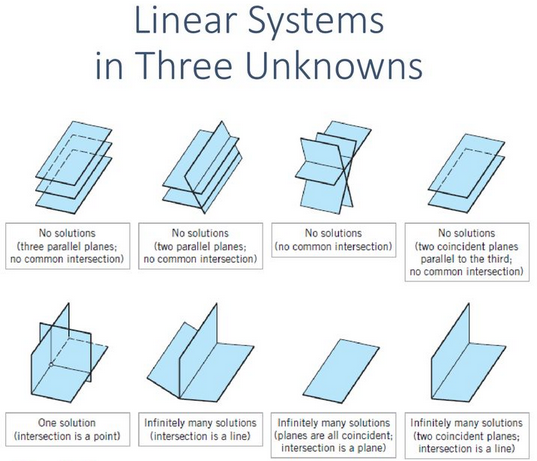
\includegraphics[width=0.8\textwidth,height=\textheight]{img/linearsystems.png}
\end{center}

\hypertarget{review-solve-the-following-systems}{%
\subsection{Review: Solve the following
systems}\label{review-solve-the-following-systems}}

\begin{enumerate}
\def\labelenumi{\arabic{enumi}.}
\item
  \systeme{2x+y=10, 3x-y=5}

  \begin{align*}
  5x &= 15 \\
  x &= 3 \\
  2(3)+y &= 10 \\
  6 + y &= 10 \\
  y &= 4
  \end{align*}
\item
  \systeme{2x+y=10, 6x+3y=10}

  \begin{align*}
  y &= 10-2x \\
  6x + 3(10-2x) &= 10 \\
  6x + 30 - 6x &= 10 \\
  30 &= 10 \therefore \text { no solution}
  \end{align*}
\item
  \systeme{5x-2y=4, 15x-6y=12}

  \begin{align*}
  0 &= 0 \\
  12 &= 12 \therefore \text{ infinite solutions}
  \end{align*}
\end{enumerate}

\begin{multicols}{2}
  \hypertarget{review-solve-the-following-systems}{%
  \subsubsection{Consistent}\label{consistent}}

  \begin{itemize}
    \tightlist
    \item A system of equations is \textbf{consistent} if it has at least one solution.
  \end{itemize}

\columnbreak

  \hypertarget{review-solve-the-following-systems}{%
  \subsubsection{Inconsistent}\label{inconsistent}}

  \begin{itemize}
    \tightlist
    \item A system of equations is \textbf{inconsistent} if it has no solutions.
  \end{itemize}

\end{multicols}

\newpage{}

\hypertarget{the-augmented-matrix}{%
\subsection{The Augmented Matrix}\label{the-augmented-matrix}}

\Large\systeme{x-y+2z=5,2x-2y+4z=10,3x-3y+6z=15}
\(\longrightarrow \left[\begin{array}{ccc|c}1 & -1 & 2 & 5 \\ 2 & -2 & 4 & 10 \\ 3 & -3 & 6 & 15 \end{array}\right]\)
\normalsize

\hypertarget{elementary-row-operations}{%
\subsection{Elementary Row Operations}\label{elementary-row-operations}}

\begin{enumerate}
\def\labelenumi{\arabic{enumi}.}
\tightlist
\item
  Interchange 2 rows
\item
  Multiply a row by a non-zero constant
\item
  Add/substract a multiple of one row to/from another row
\end{enumerate}

Doing these things changes the matrix, but it's the same system!

\hypertarget{example-1-again}{%
\subsubsection{Example 1\ldots{} again}\label{example-1-again}}

\systeme{2x+y=10, 3x-y=5}

\begin{align*}
\Large
\left[\begin{array}{cc|c}2 & 1 & 10 \\ 3 & -1 & 5 \end{array} \right]&\rowops{\frac{1}{2}R_1,}\left[\begin{array}{cc|c}1 & \frac{1}{2} & 5 \\ 3 & -1 & 5 \end{array} \right] \rowops{,R_2-3R_1}\left[\begin{array}{cc|c}1 & \frac{1}{2} & 5 \\ 0 & -\frac{5}{2} & -10 \end{array}\right] \\
&\rowops{,-\frac{2}{5}R_2} \left[\begin{array}{cc|c}1 & \frac{1}{2} & 5 \\ 0 & 1 & 4 \end{array}\right]\rowops{R1-\frac{1}{2}R_2,}\left[\begin{array}{cc|c}1 & 0 & 3 \\ 0 & 1 & 4 \end{array}\right]
\end{align*}

And so\ldots{} \(x=3\) and \(y=4\)!

\hypertarget{connection-to-matrices}{%
\subsection{Connection to Matrices}\label{connection-to-matrices}}

If we can make a system's matrix look like

\(\left[\begin{array}{ccc|c}1 & 0 & 0 & c_1 \\ 0 & 1 & 0 & c_2 \\ 0 & 0 & 1 & c_3 \end{array}\right]\),

then the solution to the system will be the ordered triple
\((c_1, c_2, c_3)\).

\hypertarget{example-2-again}{%
\subsubsection{Example 2: again}\label{example-2-again}}

\systeme{2x+y=10, 6x+3y=10}

\begin{align*}
\left[\begin{array}{cc|c}2 & 1 & 10 \\ 6 & 3 & 10 \end{array}\right] \rowops{\frac{1}{2}R1,} \left[\begin{array}{cc|c}1 & \frac{1}{2} & 5 \\ 6 & 3 & 10 \end{array}\right] \rowops{,R2-6R1,} \left[\begin{array}{cc|c}1 & \frac{1}{2} & 5 \\ 0 & 0 & -20 \end{array}\right]
\end{align*}

This is inconsistent, so there is no solution.

\hypertarget{example-3-again}{%
\subsubsection{Example 3: again}\label{example-3-again}}

\systeme{5x-2y=4, 15x-6y=12}

\begin{align*}
\left[\begin{array}{cc|c}5 & -2 & 4 \\ 15 & -6 & 12\end{array}\right]\rowops{\frac{1}{5}R1,}\left[\begin{array}{cc|c}1 & -\frac{2}{5} & \frac{4}{5} \\ 15 & -6 & 12 \end{array}\right]\rowops{,R2-15R1}\left[\begin{array}{cc|c}1 & -\frac{2}{5} & \frac{4}{5} \\ 0 & 0 & 0 \end{array}\right]
\end{align*}

Since \(0 = 0\), there are infinitely many solutions.

\hypertarget{example-4-solve-the-following-system}{%
\subsubsection{Example 4: Solve the following
system}\label{example-4-solve-the-following-system}}

\systeme{x_1-2x_2 + x_3 = 0, 2x_2-8x_3=8, -4x_1+5x_2+9x_3=-9}

\begin{align*}
&\left[\begin{array}{ccc|c}
1 & -2 & 1 & 0 \\ 0 & 2 & -8 & 8 \\ -4 & 5 & 9 & -9
\end{array}\right]\rowops{R3+4R1,}\left[\begin{array}{ccc|c}1 & -2 & 1 & 0 \\ 0 & 2 & -8 & 8 \\ 0 & -3 & 13 & -9 \end{array}\right]\rowops{,R3+\frac{3}{2}R2,}\left[\begin{array}{ccc|c}1 & -2 & 1 & 0 \\ 0 & 2 & -8 & 8 \\ 0 & 0 & -1 & 3 \end{array}\right] \\
&\rowops{,\frac{1}{2}R_2,}
\left[\begin{array}{ccc|c}
1 & -2 & 1 & 0 \\ 0 & 1 & -4 & 4 \\ 0 & -3 & 13 & -9 
\end{array}\right] \rowops{R_1+2R_2,,R_3+3R_2}\left[\begin{array}{ccc|c}
1 & 0 & -7 & 8 \\ 0 & 1 & -4 & 4 \\ 0 & 0 & 1 & 3
\end{array}\right]\rowops{R1+7R_3,R_2+4R_3,}\left[\begin{array}{ccc|c}
1 & 0 & 0 & 29 \\ 0 & 1 & 0 & 16 \\ 0 & 0 & 1 & 3
\end{array}\right]
\end{align*}

Therefore the solution to \((x_1, x_2, x_3)\) is \((29, 16, 3)\).

\hypertarget{elementary-row-operations-ref-homework-problem-08082023}{%
\subsubsection{Elementary Row Operations \& REF Homework Problem
(08/08/2023)}\label{elementary-row-operations-ref-homework-problem-08082023}}

\systeme{x + y + 2z = 8, -x - 2y + 3z = 1, 3x - 7y + 4z = 10}

\begin{align*}
&\left[\begin{array}{ccc|c}
1 & 1 & 2 & 8 \\
-1 & -2 & 3 & 1 \\
3 & -7 & 4 & 10
\end{array}\right]\rowops{,R_2+R_1,R_3-3R_1}
\left[\begin{array}{ccc|c}
1 & 1 & 2 & 8 \\
0 & -1 & 5 & 9 \\
0 & -10 & -2 & -14
\end{array}\right]\rowops{,-R_2, -R_3}\left[\begin{array}{ccc|c}
1 & 1 & 2 & 8 \\
0 & 1 & -5 & -9 \\
0 & 10 & 2 & 14
\end{array}\right] \\
&\rowops{R_1-R_2,,R_3-10R_2}\left[\begin{array}{ccc|c}
1 & 0 & 7 & 17 \\
0 & 1 & -5 & -9 \\
0 & 0 & 52 & 104
\end{array}\right]\rowops{,,\frac{1}{52}R_3}\left[\begin{array}{ccc|c}
1 & 0 & 7 & 17 \\
0 & 1 & -5 & -9 \\
0 & 0 & 1 & 2
\end{array}\right]\rowops{R_1-7R_3,R_2+5R_3,}\left[\begin{array}{ccc|c}
1 & 0 & 0 & 3 \\
0 & 1 & 0 & 1 \\
0 & 0 & 1 & 2
\end{array}\right]
\end{align*}

Therefore, the solution to \((x, y, z)\) is \((3, 1, 2)\).

\hypertarget{gaussian-elimination}{%
\subsection{Gaussian Elimination}\label{gaussian-elimination}}

\ul{Vocabulary}: A matrix is in \ul{Row Echelon Form (REF)} if:

\begin{enumerate}
\def\labelenumi{(\alph{enumi})}
\tightlist
\item
  Any rows of all zeroes are placed at the bottom of the matrix
\item
  All other rows have a \ul{leading 1} (``pivot'')
\item
  As we move down the matrix, each leading 1 is further to the right
  than the 1 above it
\end{enumerate}

A matrix is in \ul{Row Reduced Echelon Form} if the three above
conditions are met in adition to:

\begin{enumerate}
\def\labelenumi{(\alph{enumi})}
\setcounter{enumi}{3}
\tightlist
\item
  Each column with a leading 1 has all other entries in the column as a
  0. (``pivot column'')
\end{enumerate}

\newpage{}

\hypertarget{examples-1}{%
\subsubsection{Examples}\label{examples-1}}

\begin{multicols}{2}
$\begin{bmatrix}1 & 0 & 0 & 0 & 8\\ 0 & 1 & 0 & 6 & -3 \\ 0 & 0 & 1 & 7 & 10\\ 0 & 0 & 0 & 0 & 0 \end{bmatrix}$

$\begin{bmatrix}1 & 1 & 1 & 0 \\ 0 & 1 & 1 & 0 \\ 0 & 0 & 0 & 1 \end{bmatrix}$

$\begin{bmatrix}1 & 2 & -3 & 4 \\ 0 & 0 & 0 & 0 \\ 0 & 1 & 2 & -4\end{bmatrix}$
\columnbreak

REF? \checkmark \\
RREF? \checkmark \\

\vspace{1cm}

REF? \checkmark \\
RREF? \times \\

\vspace{1cm}

REF? \times \\
RREF? \times

\end{multicols}

\hypertarget{gaussian-elimination-with-back-substitution}{%
\subsection{\texorpdfstring{Gaussian Elimination With
\textbf{Back-Substitution}}{Gaussian Elimination With Back-Substitution}}\label{gaussian-elimination-with-back-substitution}}

\hypertarget{goal}{%
\subsubsection{Goal:}\label{goal}}

To get the augmented matrix in REF

Solve:
\systeme{x_1 - 2x_2 + 3x_3 = 9, -x_1 + 3x_2 = -4, 2x_1 - 5x_2 + 5x_3 = 17}
\begin{align*}
&\left[\begin{array}{ccc|c}1 & -2 & 3 & 9 \\ -1 & 3 & 0 & -4 \\ 2 & -5 & 5 & 17 \end{array}\right]\rowops{,R_2+R_1,R_3-2R_1}\left[\begin{array}{ccc|c}1 & -2 & 3 & 9 \\ 0 & 1 & 3 & 5 \\ 0 & -1 & -1 & -1 \end{array}\right]\rowops{R_1+2R_2,,R_3+R_2}\left[\begin{array}{ccc|c}1 & 0 & 9 & 19 \\ 0 & 1 & 3 & 5 \\ 0 & 0 & 2 & 4 \end{array}\right] \\
&\rowops{,,\frac{1}{2}R_3}\left[\begin{array}{ccc|c}1 & 0 & 9 & 19 \\ 0 & 1 & 3 & 5 \\ 0 & 0 & 1 & 2\end{array}\right]
\end{align*} \begin{align*}
x + 9z &= 19 \\
y + 3z &= 5 \\
z &= 2 \\
\therefore \ z &= 2, y = 5-3z, x = 19-9z \\
z &= 2, y = 5-3(2), x = 19-9(2) \\
z &= 2, y = -1, x = 1
\end{align*} Therefore, the solution \((x_1, x_2, x_3)\) is
\((1, -1, 2)\).

\hypertarget{gaussian-elimination-homework-problem-08092023}{%
\subsubsection{Gaussian Elimination Homework Problem
(08/09/2023)}\label{gaussian-elimination-homework-problem-08092023}}

\systeme{y+z-2w=-3, x+2y-z=2,2x+4y+z-3w=-2,x-4y-7z-w=-19}

\begin{align*}
&\left[\begin{array}{cccc|c}-2 & 0 & 1 & 1 & -3 \\ 0 & 1 & 2 & -1 & 2 \\ -3 & 2 & 4 & 1 & -2 \\ -1 & 1 & -4 & -7 & -19\end{array}\right]\rowops{R_4,,,R_1}\left[\begin{array}{cccc|c} -1 & 1 & -4 & -7 & -19 \\ 0 & 1 & 2 & -1 & 2 \\ -3 & 2 & 4 & 1 & -2 \\ -2 & 0 & 1 & 1 & -3\end{array}\right]\rowops{-R_1,,,} \\
&\left[\begin{array}{cccc|c} 1 & -1 & 4 & 7 & 19 \\  0 & 1 & 2 & -1 & 2 \\ -3 & 2 & 4 & 1 & -2 \\ -2 & 0 & 1 & 1 & -3\end{array}\right]\rowops{,,R_3+3R_1,R_4+2R_1}\left[\begin{array}{cccc|c} 1 & -1 & 4 & 7 & 19 \\ 0 & 1 & 2 & -1 & 2 \\ 0 & -1 & 16 & 22 & 55 \\ 0 & -2 & 9 & 15 & 35\end{array}\right]\rowops{R_1+R_2,,R_3+R_2,R_4+2R_2} \\
&\left[\begin{array}{cccc|c}1 & 0 & 6 & 6 & 21 \\ 0 & 1 & 2 & -1 & 2 \\ 0 & 0 & 18 & 21 & 57 \\ 0 & 0 & 13 & 13 & 39 \end{array}\right]\rowops{,,\frac{1}{18}R_3,}\left[\begin{array}{cccc|c}1 & 0 & 6 & 6 & 21 \\ 0 & 1 & 2 & -1 & 2 \\ 0 & 0 & 1 & \frac{7}{6} & \frac{19}{6} \\ 0 & 0 & 13 & 13 & 39 \end{array}\right]\rowops{R_1-6R_3,R_2-2R_3,,R_4-13R_3} \\
&\left[\begin{array}{cccc|c}1 & 0 & 0 & -1 & 2 \\ 0 & 1 & 0 & -\frac{10}{3} & -\frac{13}{3} \\ 0 & 0 & 1 & \frac{7}{6} & \frac{19}{6} \\ 0 & 0 & 0 & -\frac{13}{6} & -\frac{13}{6} \end{array}\right]\rowops{,,,\frac{-6}{13}R_4}\left[\begin{array}{cccc|c}1 & 0 & 0 & -1 & 2 \\ 0 & 1 & 0 & -\frac{10}{3} & -\frac{13}{3} \\ 0 & 0 & 1 & \frac{7}{6} & \frac{19}{6} \\ 0 & 0 & 0 & 1 & 1 \end{array}\right]\rowops{R_1+R_4,R_2+\frac{10}{3}R_4,R_3-\frac{7}{6}R_4,} \\
&\left[\begin{array}{cccc|c}1 & 0 & 0 & 0 & 3 \\ 0 & 1 & 0 & 0 & -1 \\ 0 & 0 & 1 & 0 & 2 \\ 0 & 0 & 0 & 1 & 1 \end{array}\right] \Longrightarrow \systeme*{w=3, x=-1, y=2, z=1}
\end{align*}



\end{document}
